\subsubsection{ARIB STD-T109}
% 
% Section about Japanese technology ARIB.
ARIB STD-T109 is a standard developed by Association of Radio Industries and Businesses, a Japanese-based organisation. The standard was developed to \textquote[\cite{2012ARIB1.0}]{\textit{Enable effective use of radio frequencies by avoiding interference among users}}, for use in intelligent transportation systems.\par
% 
The radio communication requirements for ARIB (Association of Radio Industries and Businesses) consist of single channel radio communication in the 700 MHz band with both V2I and V2V communication. The communication have to support V2V communication up to 140 km/h and V2I up to 70 km/h.\par
% 
The protocol stack of ARIB STD-t109 is of a 4 layer-structure.
Layer 1: Physical layer. It consist of 2 sublayers, physical medium dependent (PMD) sublayer and physical layer convergence protocol (PLCP) sublayer. The PMD sublayer gives a method to transmit and receive data between stations (V2I or V2V) that uses OFDM (Orthogonal frequency-division multiplexing).
Layer 2: Data link layer. It consist of 2 sublayers, MAC sublayer and LLC (Logical Link ontrol) sublayer. In the MAC sublayer CSMA/CA (Carrier sense multiple access / collision avoidance) is used for multiple access control method. The LLC sublayer lets unacknowledged services (data without error control and no guarantee of delivery) to transmit packets between upper layers.
V2V\&V2I layer: Inter-vehicle and Roadside-to-vehicle communication layer. It creates and manages data required for V2I and V2V communication control. It also makes a method to give parameters needed for communication control for the MAC sublayer (synchronises clocks etc).
Layer 7: Application layer. It gives a communication control method and services for applications such as security and It also gives a method to transmit and receive data through the V2V\&V2I layer. 
\par
The protocol data unit (PDU) of the MAC and LLC sublayer can be seen on the picture below.
\begin{figure}
    \centering
    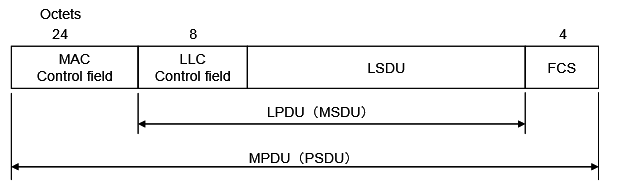
\includegraphics[width=14cm]{PSDU}
    \caption{Shows MAC protocol in parts}
    \label{fig:PSDU}
\end{figure}

A PDU of MAC called MAC protocol data unit (MPDU) consists of 4 elements. MAC Control field, LLC control field, Link service data unit (LSDU) and frame check sequence (FCS).
MAC control field's length is 24 octet and contain information needed to control and  establishing connection, it can be broken down to 6 fields with each of their length shown below.
\begin{figure}
    \centering
    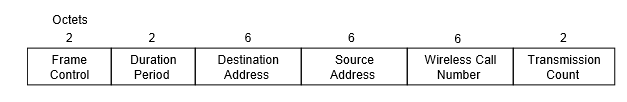
\includegraphics[width=14cm]{MAC}
    \caption{Shows breakdown of MAC Control field}
    \label{fig:MAC}
\end{figure}


Frame control has the data for what type of frames and fields is coming up. Duration period contains duration value for each frame. Destination Address is the receiver's MAC address. Source Address is the senders MAC address. Wireless call number is a identification code for security reasons. Transmission count is a number which goes up by 1 for each transmission. 

LLC control field can be split into 4 fields. DSAP address field identifies which Service Access points (SAPs) is intended for the LLC PDU. SSAP Address field identifies if the LLC PDU is a command or response PDU. Control field contains command, response, and sequence number information. Protocol identifier field sees if the right protocol is being used.
\begin{figure}[h]
    \centering
    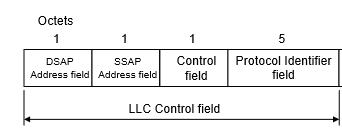
\includegraphics[width=14cm]{LLC-control-field}
    \caption{Shows breakdown of LLC control field}
    \label{fig:LLC}
\end{figure}
Lastly is the Link service data unit and Frame check sequence, which helps detect data errors that might have happened during the transmission, by checking if the number based on the data matches the FCS number, after receiving the data. 
\par
% 
Though ARIB is using the same physical layer as IEEE 802.11, one of the key differences is that the MAC address not only is being used to identify which service acess point (SAPs) of the layers but also to distinguish between communication traffic between V2V and V2I. The TDMA (Time-division multiple access) scheme is used by having control cycles of 100.000$\upmu$s which is then divided into 16 smaller cycles of  6240$\upmu$s. Each of the small cycles have 2 periods, the first period, 0 to 3024$\upmu$s is called V2I period which is the period where only that form of communication access is allowed in the channel. The reason is that the infrastructures is connected to multiple sensors scattered around the road, giving it more knowledge about the current situation than a vehicle for distributing safety information. Since each infrastructure can be allocated a specific time-slot in the V2I period, it is not necessary to use CSMA/CA. After the V2I period ends (after 3024$\upmu$s), vehicles can compete for channel access, but to avoid concurrent channel access with other vehicles, CSMA/CA is used \cite{Heinovski2016PerformanceSTD-T109}.\par
% 
Like the IEEE 802.11 and ETSI, ARIB also uses OFDM (Orthogonal Frequency Division 
Multiplexing) as modulation scheme. OFDM uses BPSK, QPSK, 16-QAM and 64-QAM\footnotemark.\par
% 
\footnotetext{\url{http://rfmw.em.keysight.com/wireless/helpfiles/n7617a/coding_and_modulation.htm}, accessed on 17/04/2017}
% 
ARIB using both TDMA and CSMA/CA (compare to 802.11p only using CSMA/CA) gives it a better communication distance in urban environment almost up to 3 times the distance \cite{Heinovski2016PerformanceSTD-T109}, because it suffers less from obstacles such as buildings etc. On the other hand, because of the priority of the V2I period, it causes packet losses for the traffic between vehicles. For same reason, message delays also happen, since they need to wait for the next time slot, which is not reserved, this causes delay in ms. 